\begin{figure}[!h]
\centering
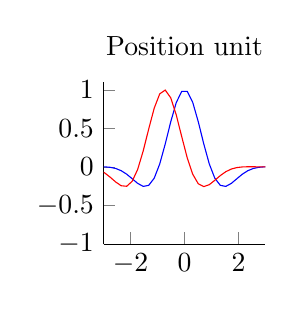
\begin{tikzpicture}[baseline]
\begin{axis}[
  width=0.3\textwidth,
  height=0.3\textwidth,
  title=Position unit,
  axis x line*=bottom,
  axis y line*=left,
  xmin=-3,xmax=3,
  ymin=-1,ymax=1.1,
  no markers,samples=50,
  ]
\addplot {exp(-0.5*(x^2)/(1^2))*cos(2*pi*15*x)};
\addplot[red] {exp(-0.5*((x+0.75)^2)/(1^2))*cos(2*pi*15*(x+0.75))};
\end{axis}
\end{tikzpicture}
%
\hskip 10pt
%
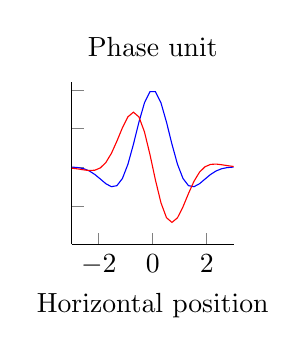
\begin{tikzpicture}[baseline]
\begin{axis}[
  width=0.3\textwidth,
  height=0.3\textwidth,
  title=Phase unit,
  axis x line*=bottom,
  axis y line*=left,
  xlabel=Horizontal position, 
  xmin=-3,xmax=3,
  ymin=-1,ymax=1.1,
  yticklabels={,,},
  no markers,samples=50]
\addplot {exp(-0.5*(x^2)/(1^2))*cos(2*pi*15*x)};
\addplot[red] {exp(-0.5*(x^2)/(1^2))*cos(2*pi*15*x + 90)};
\end{axis}
\end{tikzpicture}
%
\hskip 10pt
% 
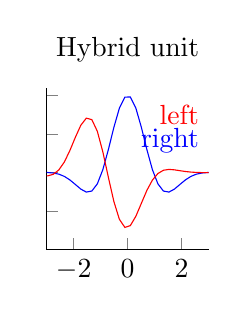
\begin{tikzpicture}[baseline]
\begin{axis}[
  width=0.3\textwidth,
  height=0.3\textwidth,
  title=Hybrid unit,
  axis x line*=bottom,
  axis y line*=left,
  xmin=-3,xmax=3,
  ymin=-1,ymax=1.1,
  yticklabels={,,},
  no markers,samples=50]
\addplot {exp(-0.5*(x^2)/(1^2))*cos(2*pi*15*x)};
\addplot[red] {exp(-0.5*((x+0.75)^2)/(1^2))*cos(2*pi*15*(x+0.75)+90)};
\node[red,above] at (axis cs:3,1) [anchor=north east] {left};
\node[blue,below] at (axis cs:3,0.7) [anchor=north east] {right};
\end{axis}
\end{tikzpicture}
\caption{One dimensional illustration of disparity encoding via position, phase, or hybrid shifts.}
\label{fig:DispEnc}
\end{figure}
